%%%%%%%%%%%%%%%%%%%%%%%%%%%%%%%%%%%%%%
% This is the name of the style file.
%%%%%%%%%%%%%%%%%%%%%%%%%%%%%%%%%%%%%%
%
% phd  -> for a PhD dissertation
% ms   -> for an MS thesis
% If both phd and ms are used then phd will overide.  If none are used,
% then ms will be active by default.
%
% cpyr -> generate a copyright page
% lof  -> generate List of Figures
% lot  -> generate List of Tables
\documentclass[ms,cpyr,lof,lot]{uathesis}

% Subsections in TOC
%% ONLY FOR PLANNING, NOT FOR FINAL COPY %%
%\setcounter{tocdepth}{4}
%\setcounter{secnumdepth}{4}

%
%%%%%%%%%%%%%%%%%%%%%%%%%%%%%%%%
% List of any packages you use.
%%%%%%%%%%%%%%%%%%%%%%%%%%%%%%%%
%

%% FROM REU SUMMARY


\usepackage{graphicx}
\usepackage{amsmath,amssymb}
%\usepackage{gensymb}
\usepackage{mathtools}
\usepackage{etoolbox}
\usepackage{booktabs}
\usepackage{float}
\usepackage{graphicx}
\usepackage{geometry}
\usepackage{multicol}
\usepackage{caption}
\usepackage{natbib}
\usepackage[outdir=./eps2pdf/]{epstopdf}
\graphicspath{
  {figures/}
  {figures/goals/}
  {figures/light_data/}
  {figures/attenuation/}
}

%%%%%%%%%%%%%%%%%%%%%%%%%%%%%%%%%%
% List of definitions you define.
%%%%%%%%%%%%%%%%%%%%%%%%%%%%%%%%%%


\DeclareMathOperator{\atantwo}{atan2}

% Domain
\newcommand\xmin{x_{\mbox{min}}}
\newcommand\xmax{x_{\mbox{max}}}
\newcommand\ymin{y_{\mbox{min}}}
\newcommand\ymax{y_{\mbox{max}}}
\newcommand\zmin{z_{\mbox{min}}}
\newcommand\zmax{z_{\mbox{max}}}

%% FROM GOALS
\newcommand\plotwidth{7in}

%% FROM REU SUMMARY

\newcommand{\ds}{\displaystyle}

% Define error function for math mode
\newcommand{\erf}{\mbox{erf}}
% Sign function
\newcommand{\sign}{\mbox{sign}}
\newcommand{\ceil}{\mbox{ceil}}
\newcommand{\floor}{\mbox{floor}}
% Real numbers
\newcommand\R{\mathbb{R}}
% Norm
\newcommand\norm[1]{||#1||}
% Length matrix entries
\newcommand\LL{\mathcal{L}}
% Frond population
\newcommand\FF{\mathcal{F}}

%% FROM RTE PAPER

% Natural numbers
\newcommand\NN{\mathbb{N}}
% Real numbers
\newcommand\RR{\mathbb{R}}
% Complex numbers
\newcommand\CC{\mathbb{C}}
% Curly B for basis
\newcommand\BB{\mathcal{B}}
% Curly D for diagonal dominance quantity
\newcommand\DD{\mathcal{D}}
\newcommand\QQ{\mathcal{Q}}
% Uniform Norm
\newcommand\unorm[1]{\left\lVert #1 \right\rVert_\infty}
% Inner Product
\newcommand\ip[1]{\left\langle #1 \right\rangle}
% Absolute value
\newcommand\abs[1]{\left| #1 \right|}
% Complex Conjugate
\newcommand\conj\overline
% Partial derivative
\newcommand\pd[2]{\frac{\partial #1}{\partial #2}}
% Iteration superscript w/ parentheses
\newcommand{\iter}[1]{^{(#1)}}
% Disable paragraph indentation
%\setlength{\parindent}{0pt}
% End of proof
\newcommand\qed{\hfill$\blacksquare$\hspace{0.5in}}

\newcommand\nomega{{n_{\vec{\omega}}}}


\title{Modelling the Light Field in Macroalgae Aquaculture}
\author{Oliver Graham Evans}
\conferraldate{May}{2018}

%The following commands specify the names and titles of people that
%will appear on the signature page.
%
%These four will always be needed.
\advisor{Dr. Kevin Kreider}
\chair{Dr. Kevin Kreider}
\collegedean{Dr. John Green}
\gradschdean{Dr. Chand Midha}
%
%For a PhD dissertation, specify a coadvisor and three committee
%members, or four committee members only.  For an MS thesis use either
%one coadvisor or one faculty reader, not both.
%
%Typical commands for a PhD dissertation (uncomment only 4).
%\coadvisor{Name of Coadvisor}
%\committee{Name of 1st Comm Member}
%\committee{Name of 2nd Comm Member}
%\committee{Name of 3rd Comm Member}
%\committee{Name of 4th Comm Member}
%
%Typical commands for an MS thesis (uncomment only 1).
\coadvisor{Dr. Curtis Clemons}
\facreader{Dr. Gerald Young}
%\facreader{Name of Fac Reader}

\begin{document}

\maketitle
\chapter{INTRODUCTION} \label{ch:intro}

\section{Motivation}
  Given the global rise in population, efficient and innovative resource utilization is increasingly important.
Future generations face major challenges regarding food, energy, and water security while addressing major issues associated with global climate change.
Growing concern for the negative environmental impacts of petroleum-based fuel is generating a market for biofuel, especially corn-based ethanol.
However, corn-based ethanol has been heavily criticized for diverting land usage away from food production, for increasing use of fertilizers that impair water quality, and for low return on energy investments for production.
At the same time, a great deal of unutilized saltwater coastline is available for both food and fuel production through seaweed cultivation.
Specifically, the sugar kelp \textit{Saccharina latissima} is known to be a viable source of food,  both for direct human consumption and biofuel production.

%TODO: Nitrogen concerns, wastewater treatment.
Nitrogen leakage into water bodies is a significant ecological problem, and is especially relevant near large conventional agriculture facilities due to run-off from nitrogen-based fertilizers, as well as near wastewater treatment plants.
Waste water treatment plants (WWTPs) in particular are facing increasingly stringent regulation of nutrients in their effluent discharges from the US Environmental Protection Agency (USEPA) and state regulatory agencies.
Nutrient management at WWTPs requires significant infrastructure, operations, and maintenance investments for tertiary treatment processes. Many treatment works are constrained financially or by space limitations in their ability to expand their treatment works.
As an alternative to conventional nutrient remediation techniques, the cultivation of the macroalgae \textit{Saccharina latissima} (sugar kelp) within the nutrient plume of WWTP ocean outfalls has been proposed.
The purpose of such an undertaking would be twofold: to prevent eutrophication of the surrounding ecosystem by sequestering nutrients, and to provide supplemental nutrients that benefit macroalgae cultivation. %TODO: Cite

Large scale macroalgae cultivation has long existed in Eastern Asia due to the popularity of seaweed in Asian cuisine, and low labor costs that facilitate its manual seeding and harvest.
  More recently, less labor-intense and more industrialized kelp aquaculture has been developing in Scandinavia and in the Northeastern United States and Canada.
For example, the MACROSEA project is a four year international research collaboration led by SINTEF, an independent research organization in Norway, and funded by the Research Council of Norway targeting ``successful and predictable production of high quality biomass thereby making significant steps towards industrial macroalgae cultivation in Norway.'' %TODO: Cite this
The project includes both cultivators and scientists, working to develop a precise understanding of the full life cycle of kelp and its interaction with its environment.
A fundamental aspect of this endeavor is the development of mathematical models to describe the growth of kelp.

Recently, a growth model\cite{broch_modelling_2012} for S. latissima has been produced and integrated into the SINMOD\cite{wassmann_modelling_2006} hydrodynamic and ecosystem model of SINTEF.
One aspect of the model which has yet to be fully developed is the availability of light, considering factors such as absorption and scattering by the aquatic medium, as well as by the kelp itself.
This thesis contributes to this effort by developing a first-principles model of the light field in a kelp farming environment.
As a first step, a model for the spatial distribution of kelp is developed.
Radiative transfer theory is then applied to determine the effects of the kelp and water on the availability of light throughout the medium.
A finite difference solution to the radiative transfer equation is developed, followed by asymptotic approximations that prove to be sufficiently accurate for clear water, and significantly less computationally intensive.
A detailed description of the numerical solution of this model is presented, accompanied by source code for a FORTRAN implementation of the solution.
This model can be used independently, or in conjunction with a kelp growth model to determine the amount of light available for photosynthesis at a single time step.

\begin{figure}[h]
  \centering
  \includegraphics[width=0.5\textwidth]{kelp_photo/sonja}
  \caption{\textit{Saccharina latissima} being harvested}
  % https://blogs.qub.ac.uk/qubio/files/2016/04/H5-5.jpg
  %TODO: Cite properly or replace with photo from Shane
\end{figure}


\section{Background on Kelp Models}

Mathematical modeling of macroalgae growth is not a new topic, although it is a reemerging one.
Several authors in the second half of the twentieth century were interested in describing the growth and composition of the macroalgae \textit{Macrocystis pyrifera}, commonly known as ``giant kelp,'' which grows prolifically off the coast of southern California.
The first such mathematical model was developed by W.J. North for the Kelp Habitat Improvement Project at the California Institute of Technology in 1968 using seven variables.
By 1974, Nick Anderson greatly expanded on North's work, and created the first comprehensive model of kelp growth which he programmed using FORTRAN\cite{anderson_mathematical_1974}.
In his model, he accounts for solar radiation intensity as a function of time of year and time of day, and refraction on the surface of the water.
He uses a simple model for shading, simply specifying a single parameter which determines the percentage of light that is allowed to pass through the kelp canopy floating on the surface of the water.
He also accounts for attenuation due to turbidity using Beer's Law.
Using this data on the availability of light, he calculates the photosynthesis rates and the growth experienced by the kelp.

Over a decade later in 1987, G.A.
Jackson expanded on Anderson's model for \textit{Macrocystis pyrifera}, with an emphasis on including more environmental parameters and a more complete description of the growth and decay of the kelp\cite{jackson_modelling_1987}. 
The author takes into account respiration, frond decay, and sub-canopy light attenuation due to self-shading.
Light attenuation is represented with a simple exponential model, and self-shading appears as an added term in the decay coefficient.
The author does not consider radial or angular dependence on shading. %TODO:  Check this. Was previously ambiguous.
Jackson also expands Anderson's definition of canopy shading, treating the canopy not as a single layer, but as 0, 1, or 2 discrete layers, each composed of individual fronds.
While this is a significant improvement over Anderson's light model, it is still rather simplistic.

Both Anderson's and Jackson's model were carried out by numerically solving a system of differential equations over small time intervals.
In 1990, M.A. Burgman and V.A. Gerard developed a stochastic population model\cite{burgman_stage-structured_1990}.
This approach is quite different, and functions by dividing kelp plants into groups based on size and age and generating random numbers to determine how the population distribution over these groups changes over time based on measured rates of growth, death, decay, light availability, etc.
In the same year, Nyman et. al. published a similar model alongside a Markov chain model, and compared the results with experimental data collected in New Zealand\cite{nyman_macrocystis_1990}.

In 1996 and 1998 respectively, P. Duarte and J.G. Ferreira used the size-class approach to create a more general model of macroalgae growth, and Yoshimori et. al. created a differential equation model of \textit{Laminaria religiosa} with specific emphasis on temperature dependence of growth rate\cite{duarte_model_1997,yoshimori_mathematical_1998}.
These were the some of the first models of kelp growth that did not specifically relate to \textit{Macrocystis pyrifera} (``giant kelp''). 
Initially, there was a great deal of excitement about this species due to it's incredible size and growth rate, but difficulties in harvesting and negative environmental impacts have caused scientists to investigate other kelp species. % TODO: Cite

\section{Background on Radiative Transfer}
In terms of optical quantities, of primary interest is in the radiance at each point from all directions, which affects the photosynthetic rate of the kelp, and therefore the total amount of biomass producible in a given area as well as the total nutrient remediation potential.
The equation governing the radiance throughout the system is known as the radiative transfer equation (RTE), which has been largely unutilized in the fields of oceanography and aquaculture.
The radiative transfer equation has been used primarily in stellar astrophysics; it's application to marine biology is fairly recent\cite{mobley_radiative_2001}.
In its full form, radiance is a function of 3 spatial dimensions, 2 angular dimensions, and frequency, making for an incredibly complex problem. % TODO: Cite?
In this work, frequency is ignored, only monochromatic radiation is considered.
The RTE states that along a given path, radiance is decreased by absorption and scattering out of the path, while it is increased by emission and scattering into the path.
In our situation, emission is negligible, owing only perhaps to some small luminescent phytoplankton or other anomaly, and can therefore be safely ignored.

% TODO: Remove?
Understanding the growth rate and nutrient recovery by
kelp cultures has important marine biological implications. For example, recent
work by our research group at Clarkson University, the University of Maine, and
SINTEF Fisheries and Aquaculture is investigating kelp aquaculture as a means to
recover nutrients from wastewater effluent plumes in coastal environments into a
valuable biomass feedstock for many products. Current models for kelp growth
place little emphasis on the way in which nearby plants shade one another.
Self-shading may be a significant model feature, though, as light availability
may impact the growth and composition of the kelp biomass, and thus the mixture
of goods that may be derived.

\section{Overview of Thesis}
% TODO: Check for redundancy
The remainder of this document is organized as follows.
In Chapter \ref{chap:kelp}, probabilistic model is developed to describe the spatial distribution of kelp by assuming simple distributions for the lengths and orientations of fronds.
Chapter \ref{chap:light} begins with a survey of fundamental radiometric quantities and optical properties of matter.
The spatial kelp distribution from Chapter \ref{chap:kelp} is used to determine optical properties of the combined water-kelp medium,
and the radiative transfer equation, an integro-partial differential equation which describes the the light field as a function of position and angle, is discussed.
An asymptotic expansion is explored for cases where absorption dominates scattering in the medium, such as in very clear water or high kelp density.
In Chapter \ref{chap:numerical}, details are given for the numerical solution of the equations from Chapters \ref{chap:kelp} and \ref{chap:light}.
Both the full finite difference solution and the asymptotic approximation are described.
Next, in Chapter \ref{chap:parameters}, the availability of necessary parameters in the literature is discussed.
For those which are not readily available, give rough estimates are given or describe experimental methods for their determination are described.
Then, in Chapter \ref{chap:model_analysis}, necessary grid resolution for adequate accuracy in the full finite difference solution is determined.
The finite difference solution is compared to the asymptotic approximation for a few sets of optical properties.
Further, we showcase the effect of varying a few key parameters on the light field predicted by the asymptotic approximation.
Afterwards, the light model developed here is used in a numerical simulation of kelp growth, and the predicted light field and biomass production are compared to those predicted by a simpler 1D exponential decay light model.
Finally, Chapter \ref{chap:conclusion} concludes the thesis by giving a brief summary of the model, discuss and its performance, and suggest improvements and avenues for future work.

\chapter{KELP MODEL}
\label{label:kelp}

\section{Physical Setup}
Being a salt water species, macroalgae cultivation occurs primarily in the ocean, with the exception of the initial stage of growth, where microscopic kelp spores are inoculated onto a thread in a small laboratory pool.
This thread is then wrapped around a large rope, which is placed in the ocean and generally suspended by buoys in one of two configurations: horizontal or vertical.
Thus far, I am primarily concerned with modeling the vertical rope case, in which the kelp plants extend radially outward from the rope in all directions, which are made up of a single frond (leaf), stipe (stem) and holdfast (root structure).
We consider a rectangular grid of such vertical ropes. 
Plants extending from each rope will shade both themselves and their neighbors
to varying degrees based on the depth of the kelp, the rope spacing, the angle
of incident light on the surface and the nature of scattering in the water.
In addition, light will be naturally absorbed by the water to varying degrees as determined by the clarity of the water.

\begin{figure}[H]
	\centering
	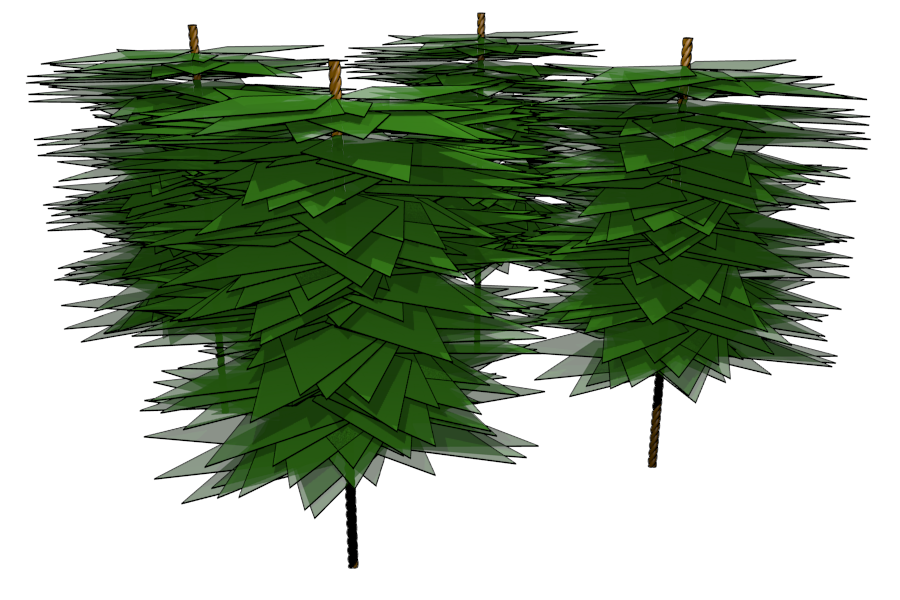
\includegraphics[width=3.5in]{kelp_array}
	\captionof{figure}{$4\times 4$ array of vertical kelp ropes}
\end{figure}
\subsection{Coordinate System}

Consider the rectangular domain
\begin{align*}
  \xmin &\leq x \leq \xmax, \\
  \ymin &\leq y \leq \ymax, \\
  \zmin &\leq z \leq \zmax.
\end{align*}
For all three dimensional analysis, we use the absolute coordinate system defined in figure \ref{fig:3dcoords}.
In the following sections, it is necessary to convert between Cartesian and spherical coordinates, which we do using the relations
\begin{align}
	\begin{split}
		x & = r\sin\phi\cos\theta, \\
		y & = r\sin\phi\sin\theta, \\
		z & = r\cos\phi. \\
	\label{eqn:coords}
	\end{split}
\end{align}

Therefore, for some function $f(x,y,z)$, we can write its derivative along a path in spherical coordinates in terms of Cartesian coordinates using the chain rule.
\begin{equation}
	\frac{\partial f}{\partial r} 
	=\frac{\partial f}{\partial x}\frac{\partial x}{\partial r} 
	+ \frac{\partial f}{\partial y}\frac{\partial y}{\partial r} 
	+ \frac{\partial f}{\partial z}\frac{\partial z}{\partial r}
\end{equation}
Then, calculating derivatives from \eqref{eqn:coords} yields
\begin{equation}
	\frac{\partial f}{\partial r} 
	=\frac{\partial f}{\partial x}\sin\phi\cos\theta
	+ \frac{\partial f}{\partial y}\sin\phi\sin\theta
	+ \frac{\partial f}{\partial z}\cos\phi.
	\label{eqn:partials}
\end{equation}
\begin{figure}[H]
	\centering
	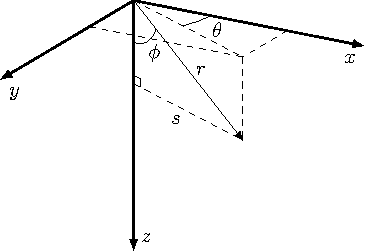
\includegraphics[width=3in]{3d_coords}
	\caption{Downward-facing right-handed coordinate system with radial distance $r$ from the origin, distance $s$ from the $z$ axis, zenith angle $\phi$ and azimuthal angle $\theta$}
	\label{fig:3dcoords}
\end{figure}


\section{Kelp Model}

\subsection{Frond shape}
\label{sec:shape}

% \begin{figure}[h]
%   \centering
%   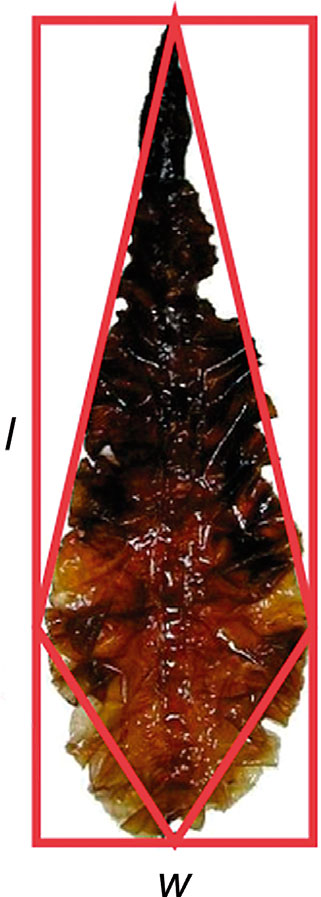
\includegraphics[width=0.7\textwidth]{kelp_photo/kite}
%   \caption{Kite-like shape of \textit{Saccharina Latissima}}
% \end{figure}

\begin{figure}[h]
	\centering
  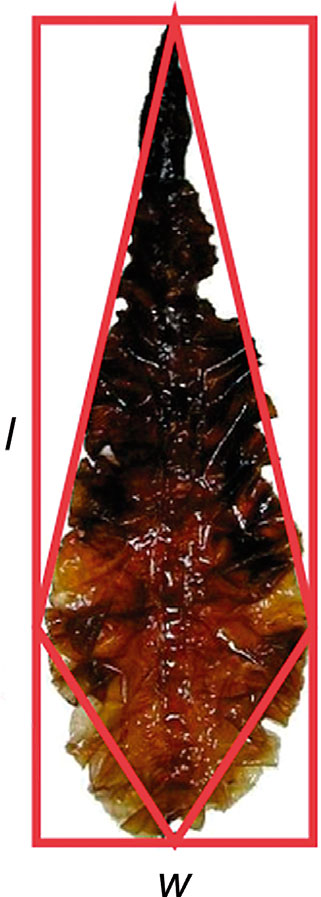
\includegraphics[width=1.2in]{kelp_photo/kite}
  %TODO: Cite this?
  \qquad
	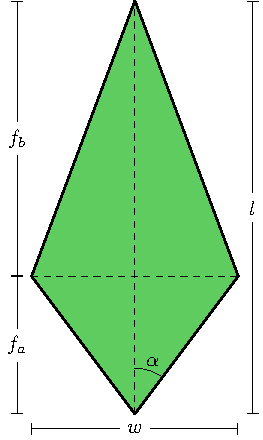
\includegraphics[width=2in]{frond}
	\captionof{figure}{Simplified kite-shaped frond}
	\label{fig:frond}
\end{figure}

We assume the frond is a kite with length $l$ from base to tip, and width $w$ from left to right.
 %In figure \ref{fig:frond}, the base is shown at the bottom and the tip is shown at the top.
 The shortest distance from the base to the diagonal connecting the left and right corners is called $f_a$, and the shortest distance from that diagonal to the tip is called $f_b$.
 We have
 \begin{equation}
	 f_a + f_b = l
 \end{equation}
When considering a whole population with varying sizes, it is more convenient to specify ratios than absolute lengths.
Let the following ratios be defined.
\begin{align}
	f_r &= \frac{l}{w} \\
	f_s &= \frac{f_a}{f_b}
\end{align}
These ratios are assumed to be consistent among the entire population, making all fronds geometrically similar.
With these definitions, the shape of the frond can be fully specified by $l$, $f_r$, and $f_s$.
It is possible, then, to redefine $w$, $f_a$ and $f_b$ as follows from the preceding formulas.

\begin{align}
	w &= \frac{l}{f_r} \\
	f_a &= \frac{lf_s}{1+f_s} \\
	f_b &= \frac{l}{1+f_s}
\end{align}

The angle $\alpha$, half of the angle at the base corner, is also important in our analysis.
Using the above equations,
\begin{equation}
	\alpha = \tan^{-1}\left(\frac{2f_rf_s}{1+f_s}\right)
\end{equation}

The area of the frond is given by
\begin{equation}
  A = \frac{lw}{2} = \frac{l^2}{2f_r}.
\end{equation}

Likewise, if the area is known, then the length is
\begin{equation}
  l = \sqrt{2Af_r}
  \label{eqn:length-from-area}
\end{equation}

\subsection{Length and angle distributions}
\label{sec:angle_dist}
We assume that frond lengths are normally distributed with mean $\mu_l$ and standard deviation $\sigma_l$.
We assume the frond angle varies according to the von Mises distribution, which is the periodic analogue of the normal distribution, defined on $[-\pi,\pi]$ rather than $(-\infty,\infty)$.
The von Mises distribution has two parameters, $\mu$ and $\kappa$, which shift and sharpen its peak respectively, as shown in Figure \ref{fig:vonmises}.
$\kappa$ can be considered analogous to $1/\sigma$ in the normal distribution.
Here, we use $\mu = \theta_w$ and $\kappa = v_w$.
That is, in the case of zero current velocity, the frond angles are be distributed uniformly, while as current velocity increases, they become increasingly likely to be pointing in the direction of the current.
Note that $\theta_w$ and $v_w$ vary over depth.

The PDF for this distribution is
\begin{equation}
	P_{\theta_f}(\theta_f) = \frac{\exp\left(v_w\cos(\theta_f-v_w)\right)}{2\pi I_0(v_w)}
\end{equation}
where $I_0(x)$ is the modified Bessel function of the first kind of order 0.
Notice that unlike the normal distribution, the von Mises distribution approaches a \textit{non-zero} uniform distribution as $\kappa$ approaches 0.
\begin{equation}
	\displaystyle \lim_{v_w \to 0}P_{\theta_f}(\theta_f) = \frac{1}{2\pi} \;\forall\, \theta_f \in [-\pi,\pi]
\end{equation}

\begin{figure}[h]
	\centering
	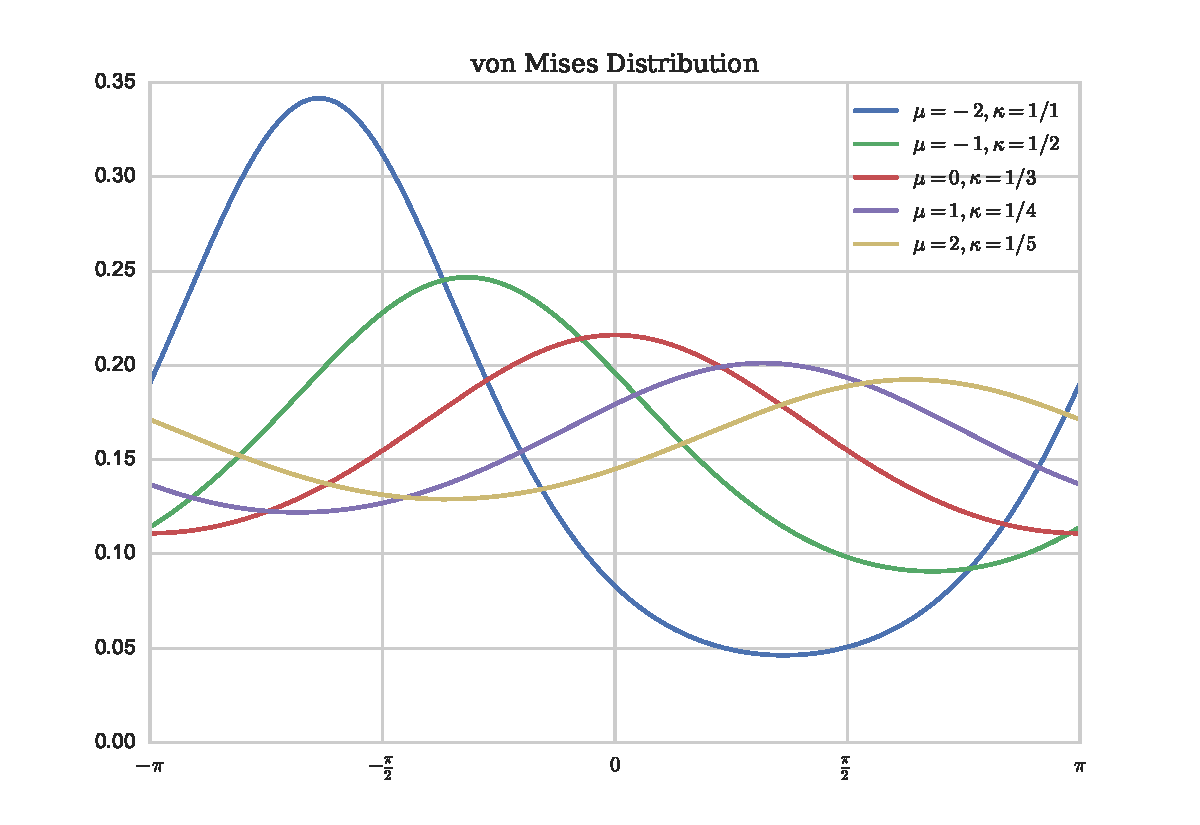
\includegraphics[width=.75\linewidth]{vonmises_2}
	\captionof{figure}{von Mises distribution for a variety of parameters}
	\label{fig:vonmises}
\end{figure}

\subsection{Combined 2D length-angle distribution}
\label{sec:2d_dist}
The previous two distributions can reasonably be assumed to be independent of one another. That is, the angle of the frond does not depend on the length, or vice versa.
Therefore, the probability of a frond simultaneously having a given frond length and angle is the product of their individual probabilities.

Given independent events $A$ and $B$,
\begin{equation}
	\label{eq:ind_prob}
	P(A \cap B) = P(A)P(B)
\end{equation}
Then the probability of frond length $l$ and frond angle $\theta_f$ coinciding is 
\begin{equation}
	P_{2D}(\theta_f,l) = P_{\theta_f}(\theta_f) \cdot L(l)
\end{equation}
A contour plot of this 2D distribution for a specific set of parameters is shown in figure \ref{fig:dist_2d}, where probability is represented by color in the 2D plane.
Darker green represents higher probability, while lighter beige represents lower probability.
In figure \ref{fig:kelp_sample}, 50 samples are drawn from this distribution and plotted.

It is important to note that if $P_{\theta_f}$ were dependent on $l$, the above definition of $P_{2D}$ would no longer be valid.
For example, it might be more realistic to say that larger fronds are less likely to bend towards the direction of the current.
In this case, \eqref{eq:ind_prob} would no longer hold, and it would be necessary to use the following more general relation.
\begin{equation}
	P(A \cap B) = P(A)P(B|A) = P(B)P(B|A)
\end{equation}
This is currently not taken into consideration in this model.

\begin{figure}[h]
	\centering
	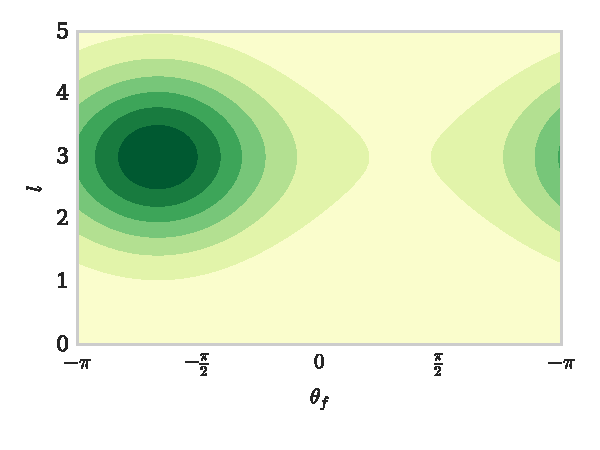
\includegraphics[width=.75\linewidth]{prob_2d}
	\vspace{-3em}
	\captionof{figure}{2D length-angle probability distribution with $\theta_w=2\pi/3,v_w=1$}
	\label{fig:dist_2d}
\end{figure}

\begin{figure}[h]
	\centering
	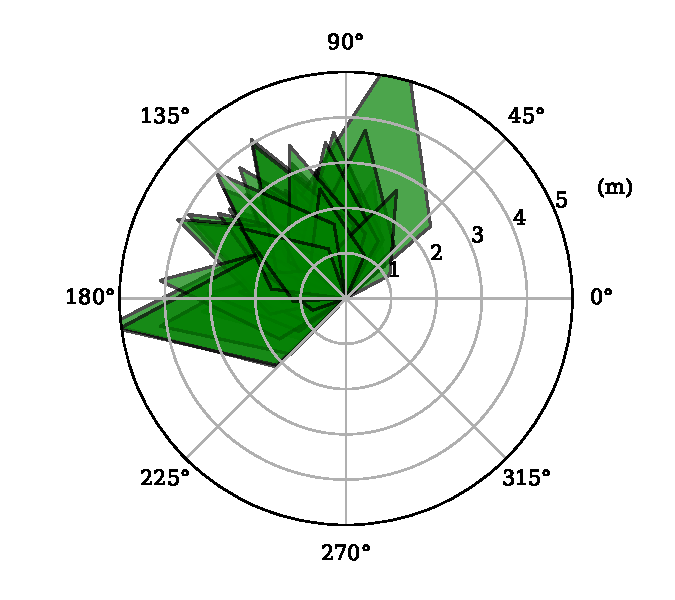
\includegraphics[width=.75\linewidth]{kelp_sample}
	\vspace{-2em}
	\captionof{figure}{A sample of 50 kelp fronds with length and angle picked from the distribution above with $f_s=0.5$ and $f_r=2$.}
	\label{fig:kelp_sample}
\end{figure}


\chapter{SOLUTION PROCEDURE}
\section{Calculate Kelp Density}
\subsection{Relative coordinate system}
\label{sec:rel_coords}
To determine under what conditions a frond will occupy a given point, we begin by
describing the shape of the frond in Cartesian and then converting to polar coordinates.
Of primary interest are the edges connected to the frond tip.
For convenience, we will use a relative coordinate system $(\theta',s)$ such that the line connecting the base to the tip is vertical, with the base at $(0,0)$.
The Cartesian analogue of this coordinate system, $(x',y')$, has the following properties.
\begin{align}
	x' &= s\cos\theta' \\ 
	y' &= s\sin\theta'
\end{align}
and
\begin{align}
	s &= \sqrt{x'^2+y'^2}
\end{align}
\vspace{-1em}
\begin{align}
	\theta' &= \atantwo(y, x)
\end{align}

\subsection{Functional description of frond edge}
With this coordinate system established, we can describe the outer two edges of the frond in Cartesian coordinates as a piecewise linear function connecting the left corner: $(-w/2,f_a)$, the tip: $(0,l)$, and the right corner: $(w/2,f_a)$.
This function has the form
\begin{equation}
	y'_f(x') = l-\sign(x')\frac{f_b}{w/2}x'.
\end{equation}

Using the equations in section \ref{sec:rel_coords}, this can be written in polar coordinates after some rearrangement as
\begin{equation}
	s_f'(\theta') = \frac{l}{\sin\theta' + S(\theta')\frac{2f_b}{w}\cos\theta'}
\end{equation}
where
\begin{equation}
	S(\theta') = \sign(\theta'-\pi/2)
\end{equation}

Then, using the relationships in section \ref{sec:shape}, we can rewrite the above equation in terms of our frond ratios $f_s$ and $f_r$.
\begin{equation}
	\label{eq:rf_rel}
	s_f'(\theta') = \frac{l}{\sin\theta' + S(\theta')\frac{2f_r}{1+f_s}\cos\theta'}
\end{equation}

\subsection{Absolute coordinates}
\label{sec:abs_coords}
To generalize to a frond pointed at an angle $\theta_f$, we will use the coordinate system $(\theta,s)$ such that
\begin{equation}
	\theta = \theta' + \theta_f - \frac{\pi}{2}
\end{equation}
Then, for a frond pointed at the arbitrary angle $\theta_f$, the function for the outer edges can be written as 
\begin{equation}
	\label{eq:rf_abs}
	s_f(\theta) = s_f'\left(\theta - \theta_f + \frac{\pi}{2} \right)
\end{equation}


\subsection{Conditions for occupancy}
Consider a fixed frond of length $l$ at an angle $\theta_f$. The point
$(\theta,s)$ is occupied by the frond if
\begin{align}
	\left|\theta_f - \theta \right| < \alpha
	\shortintertext{and}
	s < s_f(\theta)
\end{align}

Equivalently, letting the point $(\theta,s)$ be fixed, a frond occupies the point if the following conditions are satisfied.
\begin{align}
	\theta - \alpha < \theta_f < \theta + \alpha
	\label{eqn:rs_th}
	\shortintertext{and}
	l > l_{min}(\theta,s)
	\label{eqn:rs_l}
\end{align}
where
\begin{equation}
	l_{min}(\theta,s) = s \cdot \frac{l}{s_f(\theta)}
\end{equation}


Then, considering the point to be fixed, \eqref{eqn:rs_th} and \eqref{eqn:rs_l} define the spacial region $R_s(\theta,s)$ called the ``occupancy region for $(\theta,s)$'' with the property that if the tip of a frond lies within this region (i.e. $(\theta_f,l) \in R_s(\theta,s)$), then it occupies the point.
$R_s(3\pi/4,3/2)$ is shown in blue in figure \ref{fig:shade_area} and the smallest possible occupying fronds for several values of $\theta_f$ are shown in various colors.
Any frond longer than these at the same angle will also occupy the point.

\begin{figure}[h]
	\centering
	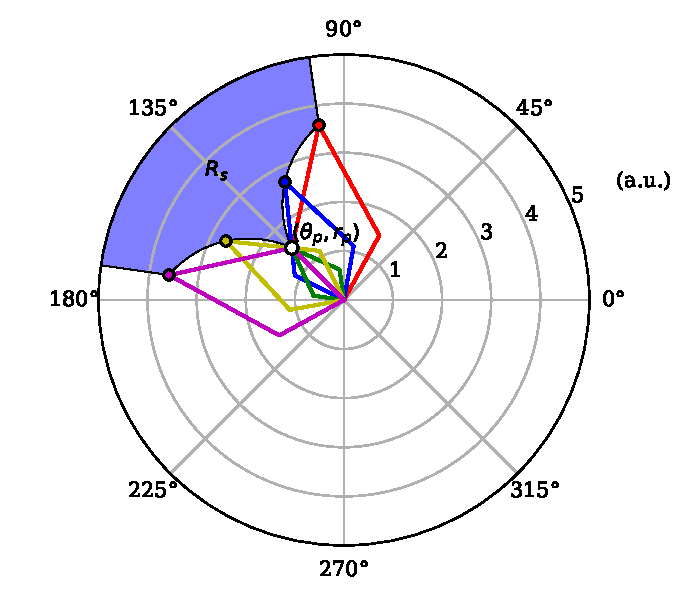
\includegraphics[width=.75\linewidth]{shade_area}
	\vspace{-2em}
	\captionof{figure}{Outlines of minimum-length fronds for a variety of angles to occupy the point $(\theta,s)=(3\pi/4,3/2)$}
	\label{fig:shade_area}
\end{figure}

\subsection{Probability of occupancy}
% TODO: Double check
We are interested in the probability that, given a fixed point $(\theta,s)$, values of $l$ and $\theta_f$ chosen from the distributions described in section \ref{sec:dist} will fall in the occupancy region.
This is found by integrating $P_{2D}$ over the occupancy region for $(\theta,s)$, as depicted in figure \ref{fig:cart_shade}.

\begin{figure}[h]
	\centering
	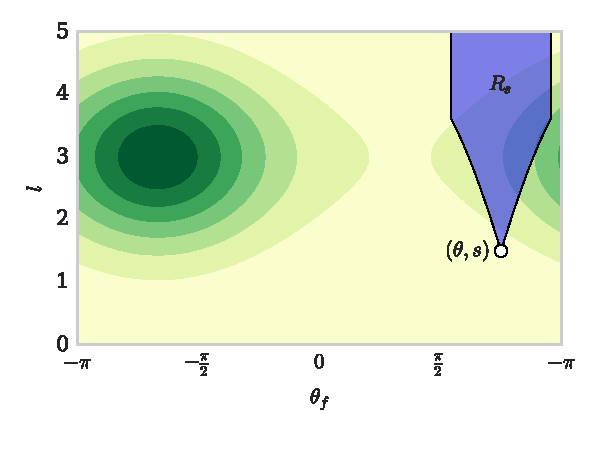
\includegraphics[width=.75\linewidth]{cart_shade}
	\vspace{-3em}
	\captionof{figure}{Contour plot of $P_{2D}(\theta_f,l)$ overlayed with the
    region in the $\theta_f-l$ plane which results in a frond occupying the point $(\theta,s)=(3\pi/4,3/2)$}
	\label{fig:cart_shade}
\end{figure}

Now, integrating $P_{2D}(\theta_f,l)$ over $R_s(\theta,s)$ yields the proportion of the population occupying the point $(\theta,s)$.
\begin{align}
		\tilde{P}_k(\theta,s,z)	&= \iint_{R_s(\theta,s)}
								P_{2D}(\theta_f,l)
								\,dl\,d\theta_f \nonumber \\
							&= \int_{\theta-\alpha}^{\theta+\alpha} 
								\int_{l_{min}(\theta_f)}^\infty
								P_{2D}(\theta_f,l)
								\,dl\,d\theta_f
\end{align}

% TODO: Revise. This is the first mention of grid cells.
Then, multiplying $\tilde{P}_k$ by the number of fronds in the population $n$ of the depth layer gives the expected number of fronds occupying the point.
Now, assuming a uniform thickness $t$ for all fronds, and a thickness $dz$ of the depth layer, we find proportion of the grid cell occupied by kelp to be
\begin{equation}
  P_k = \frac{nt}{dz}\tilde{P}.
\end{equation}

Then, the effective absorption coefficien can be calculated at any point in space as
\begin{equation}
  a(\vec{x}) = P_k(\vec{x})a_k + (1-P_k(\vec{x}))a_w
\end{equation}
% TODO: Calculate absorption coefficient grid.

\begin{figure}[h]
	\centering
	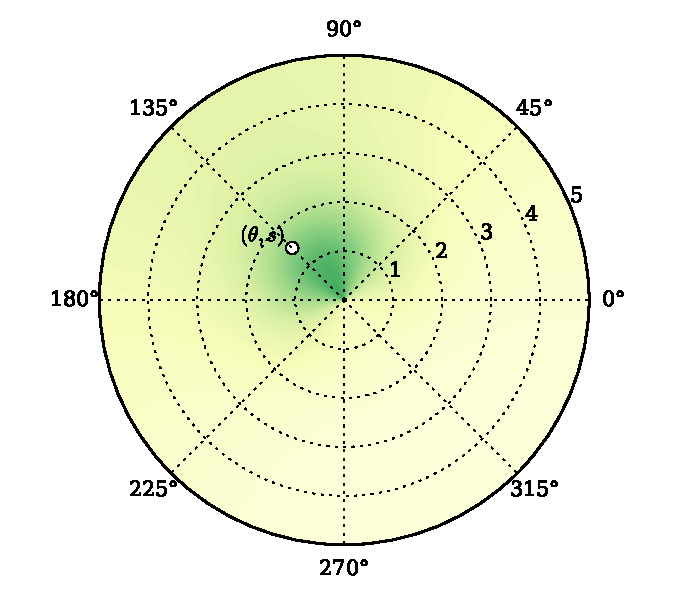
\includegraphics[width=.75\linewidth]{prob_shade}
	\vspace{-2em}
	\captionof{figure}{Contour plot of the probability of occupying sampled at 121 points using $\theta_f=2\pi/3,v_w=1$}
	\label{fig:prob_shade}
\end{figure}

\subsection{Absorbed Light}
% TODO: This.
** ADD WORDS

\newcommand{\abslight}{\mathcal{L}}
\begin{align}
  \abslight_{kq} &= \frac{dz_k}{t}
  \cdot \left(\frac{A_{kq}\mbox{ind}_{kq}}{\sum_{q'}A_{kq'}\mbox{ind}_{kq'}}\right)
  \cdot \frac{1}{\mbox{ind}_{kq}}
  \cdot \sum_{i=1}^{n_x}\sum_{j=1}^{n_y}P_{ijk}I_{ijk} \\
  &= \frac{dz_k A_{kq}}{t}
  \cdot \frac{\sum_{ij}P_{ijk}I_{ijk}}{\sum_{q'}A_{kq'}\mbox{ind}_{kq'}}
\end{align}


\section{Asymptotics}
\subsection{Substitute asymptotic series}
\newcommand{\Lasym}{L_0(\vec{x},\vec{\omega}) + b L_1(\vec{x},\vec{\omega}) + b^2 L_2(\vec{x},\vec{\omega}) + \cdots}
\newcommand{\Lasymp}{L_0(\vec{x},\vec{\omega}') + b L_1(\vec{x},\vec{\omega}') + b^2 L_2(\vec{x},\vec{\omega}') + \cdots}
\begin{align}
  L(\vec{x},\vec{\omega}) = \Lasym
\end{align}

Then, substituting the above into the RTE,

\begin{equation}
  \begin{split}
    &\vec{\omega} \cdot \nabla \left[ \Lasym \right] \\
    &+ a(\vec{x}) \left[ \Lasym \right] \\
    &= b\Bigg(
      \int_{4\pi} \beta(\abs{\vec{\omega} - \vec{\omega}'})
      \left[ \Lasymp \right] \, d\vec{\omega}' \\
    &- \left[ \Lasym \right]
    \Bigg)
    \end{split}
\end{equation}

Now, grouping like powers of $b$, we have the decoupled set of equations
\begin{align}
  \vec{\omega} \cdot \nabla L_0(\vec{x}, \vec{\omega}) + a(\vec{x})L_0(\vec{x}) &= 0 \\
  \vec{\omega} \cdot \nabla L_1(\vec{x}, \vec{\omega}) + a(\vec{x})L_1(\vec{x})
  &= \int_{4\pi} \beta(\abs{\vec{\omega} - \vec{\omega}'}) L_0(\vec{x}, \vec{\omega}')\,d\vec{\omega}' - L_0(\vec{x}, \vec{\omega}) \\ 
  \vec{\omega} \cdot \nabla L_2(\vec{x}, \vec{\omega}) + a(\vec{x})L_2(\vec{x})
  &= \int_{4\pi} \beta(\abs{\vec{\omega} - \vec{\omega}'}) L_1(\vec{x}, \vec{\omega}')\,d\vec{\omega}' - L_1(\vec{x}, \vec{\omega}) \\ 
  &\vdots \nonumber
\end{align}

\subsection{Boundary Conditions}

% TODO: Asymptotic boundary conditions
 
\subsection{Rewrite as ODE along ray path}
For all $\vec{x}, \vec{\omega}$, let
\begin{align}
  \tilde{a}(s) &= a(\vec{l}(\vec{x}, \vec{\omega}), s), \\ 
  \frac{du_0}{ds}(s) + \tilde{a}(s) u_0(s) &= 0, u_0(0) = f(\vec{\omega})
\end{align}
Then,
\begin{align}
  u_0(s) = f(\omega) \exp\left(-\int_0^s \tilde{a}(s)\, ds\right), \\
  L_0(\vec{l}(\vec{x}, \vec{\omega},s), \vec{\omega}) = u_0(s)
\end{align}

\begin{align}
  g_n(s) = \int_{4\pi} \beta(\abs{\vec{\omega} - \vec{\omega}'})
  L_{n-1}(\vec{l}(\vec{x}, \vec{\omega'}, s), \vec{\omega}')\,d\vec{\omega}' - L_{n-1}(\vec{l}(\vec{x}, \vec{\omega}, s), \vec{\omega}) \\ 
  \frac{du_n}{ds}(s) + \tilde{a}(s)u_n(s) = g_n(s), u_n(0) = 0
\end{align}

Then,
\begin{align}
  u_n(s) = \int_0^sg_n(s')\exp\left( -\int_{s''}^{s'}\tilde{a}(s'')\,ds'' \right)\, ds' \\
  L_n(\vec{l}(\vec{x}, \vec{\omega}, s), \vec{\omega}) = u_n(s)
\end{align}

\chapter{NUMERICAL IMPLEMENTATION}

In this chapter, the mathematical details involved in the numerical solution of the previously described equations.
It is assumed that this model is run in conjunction with a model describing the growth of kelp over its life cycle, which calls this light model periodically to update the light field.

\section{Kelp Numerics}

The algorithm described in this chapter has two components.
First, a probabilistic description of the kelp is generated at each point in a discrete spatial grid.
Second, optical properties of the resulting kelp-water medium are derived, and the light field is calculated.
The first component is described here.

\subsection{Length Distribution}

It is assumed that the kelp population in the lifecycle model is represented by super-individuals, as described in \citep{scheffer_super-individuals_1994}.
Rather than model each kelp frond, a subset of the population, called super-individuals, are modelled explicitly, and are considered to represent many identical iniividuals.
Specifically, at each depth $k$, we have $n$ super-individuals, indexed by $i$.
Super-individual $i$ has a frond area $A_{ki}$ and represents $n_{ki}$ individual fronds.

From \eqref{eqn:length-from-area}, the frond length of the super-individual is $l_{ki} = \sqrt{2A_{ki}f_r}$.
Given the super-individual data, we calculate the mean $\mu$ and standard deviation $\sigma$ frond
lengths using the formulas:
\begin{equation}
  \mu_k = \frac{\ds \sum_{i=1}^N l_{ki}}{\ds \sum_{i=1}^N n_{ki}},
\end{equation}
\begin{equation}
  \sigma_k = \frac{\ds \sum_{i=1}^N \left( l_{ki} - \mu_k \right)^2}{\ds \sum_{i=1}^N n_{ki}}.
\end{equation}
We then assume that frond lengths are normally distributed in each depth layer
with mean $\mu_k$ and standard deviation $\sigma_k$.

\section{Discrete Grid}
Following is a description of the uniform, rectangular spatial-angular grid used
in the numerical implementation of this model.
It is assumed that all simulated quantities are constant over the interior of a
grid cell.

The number of grid cells in each dimension are denoted by $n_x$, $n_y$, $n_z$,
$n_\theta$, and $n_\phi$, with uniform spacings $dx$, $dy$, $dz$, $d\theta$, and
$d\phi$ between adjacent grid points.

The following indices are assigned to each dimension:
\begin{align}
  x &\to i \\
  y &\to j \\
  z &\to k \\
  \theta &\to l \\
  \phi &\to m
\end{align}

It is convenient, however, to use a single index $p$ to refer to directions $\vec{\omega}$ rather than referring to $\theta$ and $\phi$ separately.
Then, the center of a generic grid cell will be denoted as
$(x_i, y_j, z_k, \vec{\omega}_p)$, and the boundaries between adjacent grid cells
will be referred to as \textit{edges}.
One-indexing will be employed throughout this document.

\subsection{Spatial Grid}
\begin{figure}[H]
  \centering
  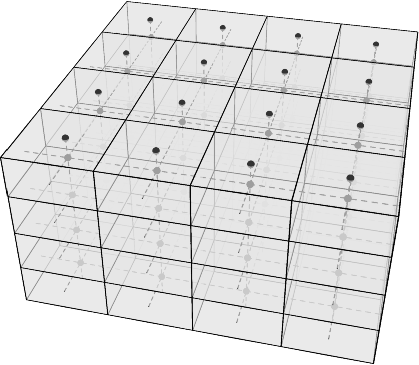
\includegraphics[width=8cm]{spatialgrid.pdf}
  \caption{Spatial grid}
  \label{fig:spatial_grid}
\end{figure}

\begin{align}
  dx &= \frac{x_{\max}-x_{\min}}{n_x} \\ 
  dy &= \frac{y_{\max}-y_{\min}}{n_y} \\ 
  dz &= \frac{z_{\max}-z_{\min}}{n_z}
\end{align}

Denote the edges as 
\begin{align}
  x_i^e &= (i-1)x \mbox{ for } i=1,\ldots,n_x \\
  y_j^e &= (j-1)y \mbox{ for } j=1,\ldots,n_y \\
  z_k^e &= (k-1)z \mbox{ for } k=1,\ldots,n_z 
\end{align}

and the cell centers as
\begin{align}
  x_i &= (i-1/2)dx \mbox{ for } i=1,\ldots,n_x \\
  y_j &= (j-1/2)dy \mbox{ for } j=1,\ldots,n_y \\
  z_k &= (k-1/2)dz \mbox{ for } k=1,\ldots,n_z
\end{align}

Note that in this convention, there are the same number of edges and cells,
and edges preceed centers.

% TODO: Not sure about this here.
Also, note that no grid center is located on the plane $z=0$.
The surface radiance boundary condition is treated separately.

\subsection{Angular Grid}
\begin{figure}[H]
  \centering
  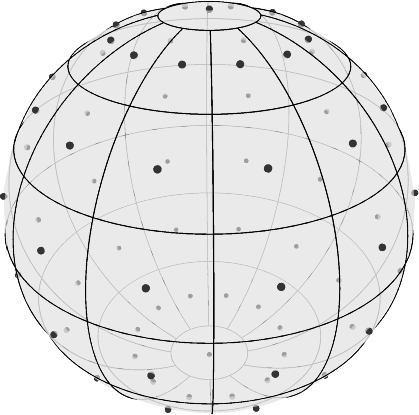
\includegraphics[width=8cm]{angulargrid.pdf}
  \caption{Angular grid}
  \label{fig:angular_grid}
\end{figure}

Now, we define the azimuthal angle such that
\begin{align}
  \theta_l = (l-1)d\theta.
\end{align}
For the sake of periodicity, we need
\begin{align}
  \theta_1 &= 0, \\
  \theta_{n_\theta} &= 2\pi-d\theta,
\end{align}
which requires
\begin{equation}
  d\theta = \frac{2\pi}{n_\theta}.
\end{equation}

A for the polar angle, we similarly let
\begin{equation}
  \phi_m = (m-1)d\phi
\end{equation}

Since the polar azimuthal is not periodic, we also store the endpoint, so
\begin{align}
  \phi_1 &= 0, \\
  \phi_{n_\phi} &= \pi.
\end{align}

This gives us
\begin{align}
  d\phi &= \frac{\pi}{n_\phi-1}.
\end{align}

It is also useful to define the edges between angular grid cells as
\begin{alignat}{3}
  \theta_l^e &= (l-1/2) d\theta, &\quad l&=1,\ldots,n_\theta \\
  \phi_m^e &= (m-1/2) d\phi, &\quad m&=1,\ldots,n_\phi-1.
\end{alignat}

Note that while $\theta$ has its final edge following its final center, this is
not the case for $\phi$.

\begin{figure}[h]
  \centering
  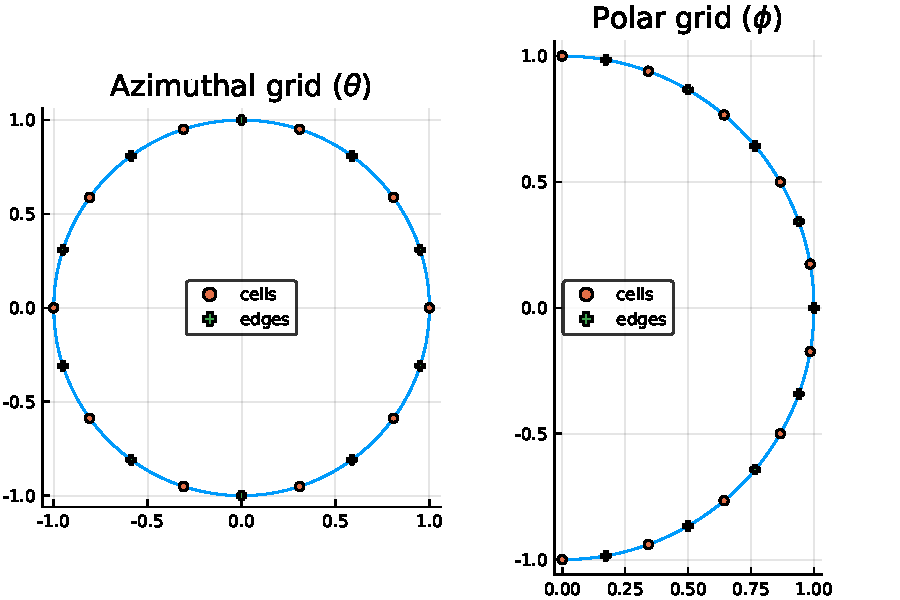
\includegraphics[width=.75\linewidth]{angular_grid_plots}
  \caption{Angular grid}
\end{figure}

As shown in Figure \ref{fig:angular_grid}, $\phi=0$ and $\phi=\pi$, called
the north ($+z$) and south ($-z$) poles respectively, are treated separately.
The total number of angles considered is $n_{\vec{\omega}} = n_\phi n_\theta -
2(n_\theta-1)$.
Since the poles create a non-rectangular angular grid in the sense that
$n_{\vec{\omega}}$ is not the product of two integers, it is advantageous to use
a single variable $p=1,\ldots,n_{\vec{\omega}}$ to index angles $\vec{\omega} =
(\theta, \phi)$ such that $p \in \left\{ 2,\ldots,n_{\vec{\omega}}-1 \right\}$ refers to the interior
of the angular grid, and $p=1$ and $p=n_{\vec{\omega}}$ refer to the
north and south poles respectively.
The following notation is used.
\begin{align}
  \hat{l}(p) &= \mbox{mod1}(p, n_\theta) \\
  \hat{m}(p) &= \ceil(p/n_\theta) + 1 \\
  \hat{\theta}_p &= \theta_{\hat{l}(p)} \\
  \hat{\phi}_p &= \phi_{\hat{m}(p)}
\end{align}

Thus, it follows that
\begin{equation}
  p = \left( \hat{m}(p)-2\right)n_\theta + \hat{l}(p).
\end{equation}

Accordingly, define
\begin{equation}
  \hat{p}(l,m) = (m-1)n_\theta + l.
\end{equation}

Further, we refer to the angular grid cell centered at $\vec{\omega}_p$ as $\Omega_p$, and the solid angle subtended by $\Omega_p$ is denoted $\abs{\Omega_p}$.
The areas of the grid cells are calculated as follows.
Note that there is a temporary abuse of notation in that the same symbols ($d\theta$ and $d\phi$) are being used for infinitessimal differential and for finite grid spacing.

For the poles, we have
\begin{align}
  \abs{\Omega_1} = \abs{\Omega_\nomega} &= \int_{\Omega_1} d{\vec{\omega}} \\
  &= \int_0^{2\pi}\int_0^{d\phi/2} \sin\phi\, d\phi\, d\theta \\
  &= 2\pi \cos\phi \Big|_{d\phi/2}^0 \\
  &= 2\pi(1-\cos(d\phi/2))
\end{align}

And for all other angular grid cells,
\begin{align}
  \abs{\Omega_p} &= \int_{\Omega_p} d{\vec{\omega}} \\
                 &= \int_{\theta_l^e}^{\theta_{l+1}^e}\int_{\phi_m^e}^{\phi_{m+1}^e} \sin(\phi)\, d\phi\, d\theta \\
                 &= d\theta \int_{\phi_m^e}^{\phi_{m+1}^e} \sin(\phi)\, d\phi \\
                 &= d\theta\left( \cos(\phi_m^e)-\cos(\phi_{m+1}^e) \right).
\end{align}


\subsection{Angular Quadrature}
We assume that all quantities are constant within a spatial-angular grid cell.
We therefore employ the midpoint rule for both spatial and angular integration.

Define the \textit{angular characteristic function}
\begin{equation}
  \mathcal{X}^\Omega_p(\vec{\omega}) = \begin{cases}
    1, & \vec{\omega} \in \Omega_p \\
    0, & \mbox{otherwise}
  \end{cases}
\end{equation}

\begin{align}
  \int_{4\pi} f(\vec{\omega})\, d\vec{\omega} &= \int_{4\pi} \sum_{p=1}^\nomega f_p \mathcal{X}^\Omega_p(\vec{\omega})\, d\vec{\omega} \\
  &= \sum_{p=1}^\nomega f_p \int_{4\pi} \mathcal{X}^\Omega_p(\vec{\omega})\, d\vec{\omega} \\
  &= \sum_{p=1}^\nomega f_p \int_{\Omega_p} d\vec{\omega} \\
  &= \sum_{p=1}^\nomega f_p \abs{\Omega_p}
\end{align}

 \subsection{Scattering Integral}

Specifically, we integrate $\beta$ to determine the amount of light scattered between angular grid cells.

Given a position $(x,y,z)$ and a direction $\vec{\omega}$, the radiance is $L_{ijkp}$.

\begin{align}
  \int_{4\pi}\beta(\vec{\omega} \cdot \vec{\omega}')f(\vec{\omega}')\, d\vec{\omega}' &= \sum_{p'=1}^\nomega f_{p'} \int_{\Omega_{p'}} \beta(\vec{\omega} \cdot \vec{\omega}')\, d\vec{\omega}' \\
\end{align}

\subsection{Discrete Variable Notation}

$L_{ijkp}$, $a_{ijk}$, $f_p$

\section{Finite Difference}

\subsection{Discretization}

For the spatial interior of the domain, we use the 2nd order central difference formula (CD2) to approximate the derivatives, which is
\begin{equation}
    \tag{CD2}
    f'(x) = \frac{f(x+dx)-f(x-dx)}{2dx} + \mathcal{O}(dx^3).
\end{equation}

When applying the PDE on the upper or lower boundary, we use the forward and backward difference (FD2 and BD2) formulas respectively.
Omitting $\mathcal{O}(dx^3)$, we have
\begin{equation}
    \tag{FD2}
    \label{eq:FD2}
    f'(x) = \frac{-3f(x)+4f(x+dx)-f(x+2dx)}{2dx}
\end{equation}
\begin{equation}
    \tag{BD2}
    \label{eq:BD2}
    f'(x) = \frac{3f(x)-4f(x-dx)+f(x-2dx)}{2dx}
\end{equation}

For the upper and lower boundaries, we need an asymmetric finite difference
method.
In general, the Taylor Series of a function $f$ about $x$ is
\begin{equation}
  f'(x+\varepsilon) = \sum_{n=1}^\infty \frac{f^{(n)}(x)}{n!} \varepsilon^n \\
\end{equation}

Truncating after the first few terms, we have
\begin{equation}
  \label{eqn:afd1}
  f'(x+\varepsilon)  = f(x) + f'(x)\varepsilon + \frac{f''(x)}{2}\varepsilon^2 + \mathcal{O}(\varepsilon^3)
\end{equation}

Similarly, replacing $\varepsilon$ with $-\varepsilon/2$ we have
\begin{equation}
  \label{eqn:afd2}
  f'(x-\frac{\varepsilon}{2}) = f(x) - \frac{f'(x)\varepsilon}{2} + \frac{f''(x)\varepsilon^2}{8} + \mathcal{O}(\varepsilon^3).
\end{equation}

Rearranging \eqref{eqn:afd1} produces
\begin{equation}
  \label{eqn:afd3}
  f''(x)\varepsilon^2 = 2f(x+\varepsilon) - 2f(x) - 2f'(x)\varepsilon + \mathcal{O}(\varepsilon^3)
\end{equation}

Combining \eqref{eqn:afd2} with \eqref{eqn:afd3} gives
\begin{align*}
  \varepsilon f'(x) &= 2f(x) - 2f(x-\frac{\varepsilon}{2}) + f''(x)\frac{\varepsilon^2}{8} + \mathcal{O}(\varepsilon^3) \\
                    &= 2f(x) - 2f(x-\frac{\varepsilon}{2}) + \frac{f(x+\varepsilon)}{4} - \frac{f(x)}{4} - \frac{f'(x)\varepsilon}{4} + \mathcal{O}(\varepsilon^3) \\
                    &= \frac{4}{5}\left( 2f(x)-2f(x-\frac{\varepsilon}{2}) + \frac{f(x+\varepsilon)}{4} - \frac{f(x)}{4} \right) + \mathcal{O}(\varepsilon^3)
\end{align*}

Then, dividing by $\varepsilon$ gives
\begin{equation}
  f'(x) = \frac{-8f(x-\frac{\varepsilon}{2}) + 7f(x) + f(x+\varepsilon)}{5\varepsilon} + \mathcal{O}(\varepsilon^2)
\end{equation}

Similarly, substituting $\varepsilon \to -\varepsilon$, we have 
\begin{equation}
  f'(x) = \frac{- f(x-\varepsilon) - 7f(x) + 8f(x+\frac{\varepsilon}{2})}{5\varepsilon} + \mathcal{O}(\varepsilon^2)
\end{equation}


\subsection{Difference Equation}

%TODO: Periodic $x,y$

In general, we have

\begin{equation}
  \vec{\omega} \cdot \nabla L_p = -(a+b) L_p + \sum_{p'=1}^{n_{\vec{\omega}}} \beta_{pp'}L_{p'}.
\end{equation}

Then,
\begin{equation}
  \vec{\omega} \cdot \nabla L_p + (a+b(1-\beta_{pp'}))L_p - \sum_{p'=1}^{n_{\vec{\omega}}} \beta_{pp'} L_{p'} = 0
\end{equation}

Interior:
\begin{equation}
  \begin{aligned}
    0 &= \frac{L_{i+1,jkp}-L_{i-1,jkp}}{2dx}\sin\hat{\phi}_p\cos\hat{\theta}_p \\
    &+ \frac{L_{i,j+1,kp}-L_{i,j-1,kp}}{2dy}\sin\hat{\phi}_p\sin\hat{\theta}_p \\
    &+ \frac{L_{ij,k+1,p}-L_{ij,k-1,p}}{2dz}\cos\hat{\phi}_p \\
    &+ (a_{ijk}+b(1-\beta_{pp'}))L_{ijkp}  - \sum_{p'=1}^{n_{\vec{\omega}}} \beta_{pp'} L_{ijkp'}
  \end{aligned}
\end{equation}

Surface downwelling (BC):
\begin{equation*}
  \begin{aligned}
    0 &= \frac{L_{i+1,jkp}-L_{i-1,jkp}}{2dx}\sin\hat{\phi}_p\cos\hat{\theta}_p \\
    &+ \frac{L_{i,j+1,kp}-L_{i,j-1,kp}}{2dy}\sin\hat{\phi}_p\sin\hat{\theta}_p \\
    &+ \frac{-8f_p + 7L_{ijkp} + L_{ij,k+1,p}}{5dz}\cos\hat{\phi}_p \\
    &+ (a_{ijk}+b(1-\beta_{pp'}))L_{ijkp} \\
    &- \sum_{p'=1}^{n_{\vec{\omega}}} \beta_{pp'} L_{ijkp'}.
  \end{aligned}
\end{equation*}

Combining $L_{ijkp}$ terms on the left and moving the boundary condition to the
right gives

\begin{equation}
  \begin{aligned}
    &\frac{L_{i+1,jkp}-L_{i-1,jkp}}{2dx}\sin\hat{\phi}_p\cos\hat{\theta}_p \\
    + &\frac{L_{i,j+1,kp}-L_{i,j-1,kp}}{2dy}\sin\hat{\phi}_p\sin\hat{\theta}_p \\
    + &\frac{L_{ij,k+1,p}}{5dz}\cos\hat{\phi}_p \\
    + &(a_{ijk}+b(1-\beta_{pp'}) + \frac{7}{5dz} \cos\hat{\phi}_p)L_{ijkp} \\
    - &\sum_{p'=1}^{n_{\vec{\omega}}} \beta_{pp'} L_{ijkp'} = \frac{8f_p}{5dz} \cos\hat{\phi}_p.
  \end{aligned}
\end{equation}

Likewise for the bottom boundary condition, we have

\begin{equation}
  \begin{aligned}
    0 &= \frac{L_{i+1,jkp}-L_{i-1,jkp}}{2dx}\sin\hat{\phi}_p\cos\hat{\theta}_p \\
    &+ \frac{L_{i,j+1,kp}-L_{i,j-1,kp}}{2dy}\sin\hat{\phi}_p\sin\hat{\theta}_p \\
    &- \frac{L_{ij,k-1,p}}{5dz}\cos\hat{\phi}_p \\
    &+ (a_{ijk}+b(1-\beta_{pp'}) - \frac{7}{5dz}\cos\hat{\phi}_p)L_{ijkp} \\
    &- \sum_{p'=1}^{n_{\vec{\omega}}} \beta_{pp'} L_{ijkp'}.
  \end{aligned}
\end{equation}

Now, for upwelling light at the first depth layer (non-BC), we apply FD2.
\begin{equation}
  \begin{aligned}
    0 &= \frac{L_{i+1,jkp}-L_{i-1,jkp}}{2dx}\sin\hat{\phi}_p\cos\hat{\theta}_p \\
    &+ \frac{L_{i,j+1,kp}-L_{i,j-1,kp}}{2dy}\sin\hat{\phi}_p\sin\hat{\theta}_p \\
    &+ \frac{-3L_{ijkp} + 4L_{ij,k+1,p} - L_{ij,k+2,p}}{2dz}\cos\hat{\phi}_p \\
    &+ (a_{ijk}+b(1-\beta_{pp'}))L_{ijkp} \\
    &- \sum_{p'=1}^{n_{\vec{\omega}}} \beta_{pp'} L_{ijkp'}.
  \end{aligned}
\end{equation}

Grouping $L_{ijkp}$ terms gives
\begin{equation}
  \begin{aligned}
    0 &= \frac{L_{i+1,jkp}-L_{i-1,jkp}}{2dx}\sin\hat{\phi}_p\cos\hat{\theta}_p \\
    &+ \frac{L_{i,j+1,kp}-L_{i,j-1,kp}}{2dy}\sin\hat{\phi}_p\sin\hat{\theta}_p \\
    &+ \frac{4L_{ij,k+1,p} - L_{ij,k+2,p}}{2dz}\cos\hat{\phi}_p \\
    &+ \left(a_{ijk}+b(1-\beta_{pp'}) - 3\frac{\cos\hat\phi_p}{2dz} \right)L_{ijkp} \\
    &- \sum_{p'=1}^{n_{\vec{\omega}}} \beta_{pp'} L_{ijkp'}.
  \end{aligned}
\end{equation}

Similarly, for downwelling light at the lowest depth layer, we have
\begin{equation}
  \begin{aligned}
    0 &= \frac{L_{i+1,jkp}-L_{i-1,jkp}}{2dx}\sin\hat{\phi}_p\cos\hat{\theta}_p \\
    &+ \frac{L_{i,j+1,kp}-L_{i,j-1,kp}}{2dy}\sin\hat{\phi}_p\sin\hat{\theta}_p \\
    &+ \frac{-4L_{ij,k-1,p} + L_{ij,k-2,p}}{2dz}\cos\hat{\phi}_p \\
    &+ \left(a_{ijk}+b(1-\beta_{pp'}) + 3\frac{\cos\hat\phi_p}{2dz} \right)L_{ijkp} \\
    &- \sum_{p'=1}^{n_{\vec{\omega}}} \beta_{pp'} L_{ijkp'}
  \end{aligned}
\end{equation}

\subsection{Structure of Linear System}

Describe layout of matrix.

Number of rows/columns: $n_xn_yn_zn_{\vec{\omega}}$

Number of nonzero RHS entries: $n_xn_yn_z/2$

** Table with number of nonzero matrix entries in each type of row (interior,
exterior-BC, exterior non-BC)

Number of nonzero matrix entries: $n_xn_yn_{\vec{\omega}} \left[n_z(n_{\vec{\omega}}+6)-1 \right]$

\section{GMRES}
GMRES is a Krylov Subspace method. These work like this. Here's what's special
about GMRES. Advantages. Drawbacks. Not practical for running in SINMOD.

\section{Numerical Asymptotics}

\subsection{Ray Tracing Algorithm}
% TODO: Revise
\subsubsection{Extract values along path}

In order to evaluate a path integral through the previously described grid, it
is first necessary to construct a one-dimensional piecewise constant integrand
which is discontinuous at unevenly spaced points corresponding to the
intersections between the path and edges in the spatial grid.

Consider a grid center $\vec{p_1} = (p_{1x},p_{1y},p_{1z})$ and a corresponding path $\vec{l}(\vec{x_1}, \vec{\omega}, s)$.
To find the location of discontinuities in the itegrand, we first calculate the
distance from its origin, $\vec{p_0} = \vec{x_0}(\vec{p_1}, \vec{\omega}) = (p_{0x}, p_{0y}, p_{0z})$ to grid edges in each dimension
separately.

Given
\begin{align}
  x_i &= p_{0x} + \frac{s_i^x}{\tilde{s}}(p_{1x}-p_{0x}) \\
  y_j &= p_{0y} + \frac{s_j^y}{\tilde{s}}(p_{1y}-p_{0y}) \\
  z_k &= p_{0z} + \frac{s_k^z}{\tilde{s}}(p_{1z}-p_{0z})
\end{align}

we have
\begin{align}
  s_i^x &= \tilde{s}\frac{x_i-p_{0x}}{p_{1x}-p_{0x}} \\
  s_i^y &= \tilde{s}\frac{y_i-p_{0y}}{p_{1y}-p_{0y}} \\
  s_i^z &= \tilde{s}\frac{z_i-p_{0z}}{p_{1z}-p_{0z}} \\
\end{align}


We also keep a record for each dimension specifying whether the ray increases
or decreases in the dimension. Let
\begin{align}
  \delta_x &= \sign(p_{0x}-p_{1x}) \\
  \delta_y &= \sign(p_{0y}-p_{1y}) \\
  \delta_z &= \sign(p_{0z}-p_{1z})
\end{align}

For convenience, we also store a closely related quantity, $\sigma$ with a value 1 for
increasing rays and 0 for decreasing rays in each dimension
\begin{align}
  \sigma_x = (\delta_x+1)/2 \\
  \sigma_y = (\delta_y+1)/2 \\
  \sigma_z = (\delta_z+1)/2
\end{align}

For this algorithm, we keep two sets of indices. $(i,j,k)$ indexes the grid
cell, and will be used for extracting physical quantities from each cell along
the path.
Meanwhile, $(i^e,j^e,k^e)$ will index the edges between grid cells, beginning
after the first cell. i.e., $i^e=1$ refers not to the plane $x=\xmin$, but to $x=\xmin+dx$.

Let $(i_0, j_0, k_0)$ be the indices of the grid cell containing $\vec{p_0}$.

That is,

\begin{align}
  i_0 &= \ceil\left(\frac{p_{0x}-\xmin}{dx}\right) \\
  j_0 &= \ceil\left(\frac{p_{0y}-\ymin}{dy}\right) \\
  k_0 &= \ceil\left(\frac{p_{0z}-\zmin}{dz}\right)
\end{align}

Then,
\begin{align}
  i_0^e &= i_0 + \sigma_x \\
  j_0^e &= j_0 + \sigma_y \\
  k_0^e &= k_0 + \sigma_z
\end{align}

Now, we calculate the distance from $p_0$ along the path to edges in each dimension.
\begin{align}
  s_i^x = \hat{s}\frac{x_i^e-p_{0x}}{p_{1x}-p_{0x}} \\
  s_j^y = \hat{s}\frac{y_j^e-p_{0y}}{p_{1y}-p_{0y}} \\
  s_k^z = \hat{s}\frac{z_k^e-p_{0z}}{p_{1z}-p_{0z}}
\end{align}

For each grid cell, we check the path lengths required to cross an $x$, $y$, and
$z$ edge-planes.
Then, we move to the next grid cell in that dimension.
That is,

* We also track $s$, the path length.

Consider $i,j,k$ fixed (denoting the current grid cell).

\begin{align}  
  d = \mbox{argmin}_{x,y,z} \left\{ s_i^x-s, s_j^y-s, s_k^z \right\}
\end{align}

Then,
* Incorrect use of left brace
\begin{align}
  \begin{cases}
    i = i+\delta_x, & \mbox{if } d=x \\
    j = j+\delta_y, & \mbox{if } d=y \\
    z = k+\delta_z, & \mbox{if } d=z
  \end{cases}
\end{align}

and

\begin{align}
  \begin{cases}
    i^e = i^e+\delta_x, & \mbox{if } d=x \\
    j^e = j^e+\delta_y, & \mbox{if } d=y \\
    z^e = k^e+\delta_z, & \mbox{if } d=z
  \end{cases}
\end{align}


Then, move to the adjacent grid cell in the dimension which requires the shortest
step to reach an edge. Save $ds$ of the path through this cell. Also save abs.
coef. and source.
** Definitely needs more work**

- absorption coefficient ($\tilde{a}(s)$)

- effective source ($g_n(s)$)

\subsubsection{Ray integral}

Here are the equations for calculating the double integral over ray paths
required for the asymptotics. It will hopefully make more sense once I add words
to accompany the symbols.

Let
\begin{align}
  g_n(s) &= \sum_{i=1}^{N-1}g_{ni}\mathcal{X}_i(s) \\
  \tilde{a}(s) &= \sum_{i=1}^{N-1}\tilde{a}_{i}\mathcal{X}_i(s) \\
\end{align}

and
\begin{equation}
  \mathcal{X}_i(s) = \begin{cases}
    1, & a_I \leq s < s_{i+1} \\
    0, & \mbox{otherwise}
    \end{cases}
\end{equation}

and $\left\{s_i\right\}_{i=1}^N$ is increasing.

Let $ds_i = s_{i+1} - s_i$.

Let $\hat{i}(s) = \min\left\{ i \in \{1,\ldots,N\} : s_i>s \right\}$.
Let $\tilde{d}(s) = s_{\hat{i}(s)}-s$.

We have $s_1 = 0$ and $s_N = \tilde{s}$.


\begin{align}
  u_n(\tilde{s}) &= \int_0^{\tilde{s}}g_n(s')\exp\left( -\int_{s''}^{s'}\tilde{a}(s'')\,ds'' \right)\, ds' \\
  &= \int_0^{s_N} \sum_{i=1}^{N-1}g_{ni}\mathcal{X}_i(s') \exp\left( -\int_{s''}^{s'}\sum_{j=1}^{N-1}\tilde{a}_{j}\mathcal{X}_j(s'')\,ds'' \right)\, ds' \\
  &= \sum_{i=1}^{N-1}g_{ni}\int_0^{s_N} \mathcal{X}_i(s') \exp\left( -\sum_{j=1}^{N-1}\tilde{a}_{j}\int_{s''}^{s'}\mathcal{X}_j(s'')\,ds'' \right)\, ds' \\
  &= \sum_{i=1}^{N-1}g_{ni}\int_{s_i}^{s_{i+1}}  \exp\left(-\tilde{a}_{\hat{i}(s')-1}\tilde{d}(s') -\sum_{j=\hat{i}(s')}^{N-1}\tilde{a}_{j}ds_j\right)\, ds' \\
  &= \sum_{i=1}^{N-1}g_{ni}\int_{s_i}^{s_{i+1}}  \exp\left(-\tilde{a}_{i}(s_{i+1}-s') -\sum_{j=i+1}^{N-1}\tilde{a}_{j}ds_j\right)\, ds'
\end{align}

Let
\begin{equation}
  b_i = -\tilde{a}_{i}s_{i+1} - \sum_{j=i+1}^{N-1}\tilde{a}_{j}ds_j.
\end{equation}

Then,
\begin{align}
  u_n(\tilde{s}) &= \sum_{i=1}^{N-1}g_{ni}\int_{s_i}^{s_{i+1}}  \exp\left(\tilde{a}_{i}s' + b_i\right)\, ds' \\
                 &= \sum_{i=1}^{N-1}g_{ni}e^{b_i}\int_{s_i}^{s_{i+1}}  \exp\left(\tilde{a}_{i}s'\right) ds'
\end{align}

Let
\begin{align}
  d_i &= \int_{s_i}^{s_{i+1}}  \exp\left(\tilde{a}_{i}s'\right)\, ds' \\
    &= \begin{cases}
    ds_i, & \tilde{a} = 0 \\
      \left( \exp(\tilde{a}_i s_{i+1}) - \exp(\tilde{a}_i s_i) \right)/\tilde{a}_i, & \mbox{otherwise}
    \end{cases}
\end{align}

Then,
\begin{equation}
  u_n(\tilde{s}) = \sum_{i=1}^{N-1} g_{ni}d_i e^{b_i}
\end{equation}

\chapter{NUMERICAL ANALYSIS} \label{ch:model_analysis}

\section{Grid Study}
Run many grid sizes with GMRES, using asymptotic solution as initial guess.
Compare CPU times and accuracy, assuming largest grid is ``true'' solution.
Determine necessary grid size to achieve reasonable accuracy.

\section{Asymptotics vs. Finite Difference}
Compare asymptotic solutions to GMRES with reasonable grid size as determined
above. Compare CPU time and accuracy. Determine ideal number of scatters to
include (number of terms in asymptotic series). Repeat for a few values of
scattering coefficient.

\section{Parameter Study}
Vary parameters and measure average differences in radiance for full grid, as
well as average irradance over depth.

- absorption coefficient

- scattering coefficient

- VSF

- frond bending coefficient
\chapter{EXPERIMENTAL DETERMINATION OF PARAMETERS} \label{ch:experiment}

It looks like we probably won't be able to get the synthetic kelp to actually do
the experiments, but I'll describe what one would do in order to determine
``frond bending coefficients'', as well as optical properties of water and kelp,
citing literature and reporting values obtained by others.


\section{Parameters from Literature}
\begin{table}
  \caption{Parameter values}
  \centering
  \begin{tabular}{p{2\textwidth/7} p{\textwidth/7} p{\textwidth/6} p{\textwidth/6} p{2\textwidth/7}}
    \toprule
    Parameter Name & Symbol & Value(s) & Citation & Notes \\
    \midrule
    Kelp Absorptance & $A_k$ & 0.8 & \cite{colombo-pallotta_photosynthetic_2006} & Actually for \textit{Macrocystis Pyrifera}\\
    Scattering coefficient & $b$ & 0.366 & \cite{sokolov_parameterization_2010} & Table 2, $b_{\lambda 0}$, mean \\
    VSF & $\beta$ & tabulated & \cite{petzold_volume_1972,sokolov_parameterization_2010}, & Currently using Petzold\\ 
    \bottomrule
  \end{tabular}
\end{table}


\section{Optical Properties}
\subsection{Absorption Coefficients}
\subsection{Scattering Coefficients}
\subsection{Volume Scattering Function}

\section{Frond Distribution Parameters}
\subsection{Rotation}
\subsection{Lift}

\chapter{SIMULATION RESULTS}

Run Ole Jacob's model with my new light model, compare:

- irrad over time for several depths

- computation time

- harvestable biomass
\chapter{CONCLUSION}

It was great and I've survived so far. Does future work go here?
\bibliographystyle{abbrv}
\bibliography{bio}
%If you have n appendices, then use the \appendices{n} command below
%followed by n \input{filename} commands, similar to the \input{chapx}
%commands above.
% DO NOT USE SECTIONS OR SUBSECTIONS IN AN APPENDIX OR APPENDICES
% \appendix{3}
% \chapter{APPENDIX TITLE GOES HERE} \label{ap:a}


{\bf DO NOT SECTION OR SUBSECTION AN APPENDIX OR APPENDICS}

We will recylcle Chapters~\ref{2DWaveEquation} and \ref{TabAndFigChap}
to make the following two appendices.


%%%%%%% DO NOT SECTION APPENDICES





% \chapter{SECOND APPENDIX: THE TWO DIMENSIONAL WAVE EQUATION} \label{ap:2DWaveEquation}

{\bf  DO NOT SECTION OR SUBSECTION AN APPENDIX OR APPENDICES}

A series solution for the two-dimensional wave equation
\begin{equation}
\frac{1}{c^{2}}\frac{\partial^{2}u}{\partial t^{2}} = \frac{\partial^{2}u}{\partial r^{2}} + %
        \frac{1}{r}\frac{\partial u}{\partial r} + \frac{1}{r^{2}}\frac{\partial^{2}u}%
        {\partial\theta^{2}}                                                                 \label{ap:waveEq}
\end{equation}
for outgoing waves is
\begin{equation}
u = \sum_{n=0}^{\infty}a_{n}(\theta)f^{n}(r,t),                                              \label{ap:Soln}
\end{equation}
where
\begin{equation}
f^{n} = \sum_{k=0}^{\infty}r^{-k-\frac{1}{2}}f_{k}^{n}(ct-r).                                \label{ap:function}
\end{equation} %look up reference.

You can reference a labeled equation by using the \textit{ref}
command.  For example, you can show that equations (\ref{ap:Soln}) and
(\ref{ap:function}) are a solution to equation (\ref{ap:waveEq}).
(see the file chap2.tex for the commands).



% \chapter{EXAMPLE OF A TABLE AND A FIGURE} \label{ap:TabAndFigChap}

{\bf DO NOT SECTION OR SUBSECTION AN APPENDIX OR APPENDICES}

\begin{table}[h]
\begin{center}
\caption{Table captions belong above the table} \label{ap:tb:disc}
\vskip .1 truein
\begin{tabular}{|l||c||c||c|} \hline \hline
\textbf{Name} & \textbf{Variable} & \textbf{Discretization} & \textbf{Step} \\ \hline
Radius      &       $r\in[a,R]$      &          $r_{k} =a + k dr,\quad k=0,1,2,\dots,K$   &    $dr = (R-a)/K$  \\ \hline
Angle       &       $\theta\in[0,2\pi)$ &      $\theta_{l} = l d\theta, \quad l =0,1,2,\dots,L-1$ & $d\theta = 2\pi/L$ \\ \hline
Time         &       $t\in[0,T]$           &      $t_{p} = p dt, \quad p =0,1,2,\dots,P$     &     $dt = T/P$ \\ \hline \hline
\end{tabular}
\end{center}
\end{table}

\begin{figure}[h]
\begin{center}
\includegraphics[width=3in,angle=-90]{Waves.eps}
\end{center}
\caption{Figure labels go below the figure} \label{ap:fg:N5Wave}
\end{figure}

To include figures side-by-side use the minipage environment.

\begin{figure}[ht]
\begin{minipage}{0.45\linewidth}
\begin{center}
\includegraphics[width=2.25in,angle=-90]{Waves.eps}
\vspace{0in}\ref{ap:sbys}A:
\end{center}
\end{minipage} \hfill
\begin{minipage}{0.45\linewidth}
\begin{center}
\includegraphics[width=2.25in,angle=-90]{Waves.eps}
\vspace{0in}\ref{ap:sbys}B:
\end{center}
\end{minipage}
\caption{Figures side-by side}\label{ap:sbys}
\end{figure}

See chap4.tex for the commands used to build the table and figure.  As
you add chapters, figures, and tables, the table of contents and lists
will automatically be updated.

Figure~\ref{ap:sbys} is an example of figures side-by-side, with
Figure~\ref{ap:sbys}A to the left of \ref{ap:sbys}B.


\end{document}
